\chapter{Methods}
\label{chapterlabel2}

\section{Calibrations of ultrasonic transducers}
\begin{itemize}
    \item Where do I need to describe the whole ultrasonic measuring system.
    \item Bottom plug with x number of lead-through cables made of some material.
    \item Pulsing, amplification and receiving. 
    \item include diagram of sensors and description of how they are made.
    \item i.e. cable soldered to metal conductive end and ceramic placed into aluminium end which has a concave face to fit to circumference of the sample, end screws onto cap and is tightened with grounding wire acts as a "spring" to give a good contact of the crystal.
    \item Include details of piezoelectric ceramics. 
    \item p-wave: disk shaped with a diameter of x mm and a thickness of x mm made by x company which have a frequency of x MHz.
    \item sh-wave: disk shaped with a diameter of x mm and a thickness of x mm made by x company which have a frequency of x MHz.
\end{itemize}



Using aluminium sample of 40 mm diameter we arranged 8 p-wave transducers and 6 sh-wave transducers around the circumference in a formation allowing for p-waves to be recorded at 5 angles and sh-waves at 3 angles.


\section{Calibrations of pore fluid system storage capacity}
\begin{itemize}
    \item Need to have already described pore pressure system or do it here.
    \item Include a schematic of the fluid pressure pipes and values.
    \item Describe the processing of increasing and decreasing pore pressure with a different combination of values open and closed.
    \item Assumes that the valves are zero fluid volume.
    \item Discuss that the storage capacity is a function of fluid pressure and also a function of the position of the piston in the intensifier ("pore volume" that is measured on system).
\end{itemize}

The units of measurement of the storage capacity of the dead volume are m$^3$Pa$^{-1}$. The calibration is achieved by measuring the change in fluid volume on the pore pressure intensifier following changes in pore pressure. The storage of the dead volume depends on the type of fluid, the fluid pressure, and the nominal pore volume (the position of the piston in the intensifier). Therefore, calibration is conducted for the same fluid (water), fluid pressure (around 10 MPa), and pore volume levels as were used during the experiments.

Measuring small changes in pore volume are difficult as volume changes appear to be non-linear at small resolution. This could be due to stick-slip behaviour of the pore pressure intensifier. RATE AND STATE FRICTION: I SHOULD TEST WHETHER THIS IS STILL THE CASE WHEN FLUID PRESSURE IS VARIED QUICKLY. THIS IS NOT REALLY IMPORTANT FOR MY STUFF BECAUSE PORE FLUID DIFFUSES INTO THE DEAD VOLUME RELATIVELY SLOWLY. Small changes in fluid pressure do not result in similar changes in measured pore volume around the same pore pressure levels. I.e. local gradients of the fluid pressure - intensifier volume curve can vary dramatically from the general trend. The behaviour of the intensifier fluid volume change to fluid pressure change is repeatable whether increasing or decreasing pressure (good). Also, the local stick-slip like behaviour consistently occurs at the same position of the fluid volume intensifier, even if fluid pressure differs. Therefore, it is understood that there is a physical reason to explain this, perhaps scratches on the piston.

\begin{figure}
    \centering
    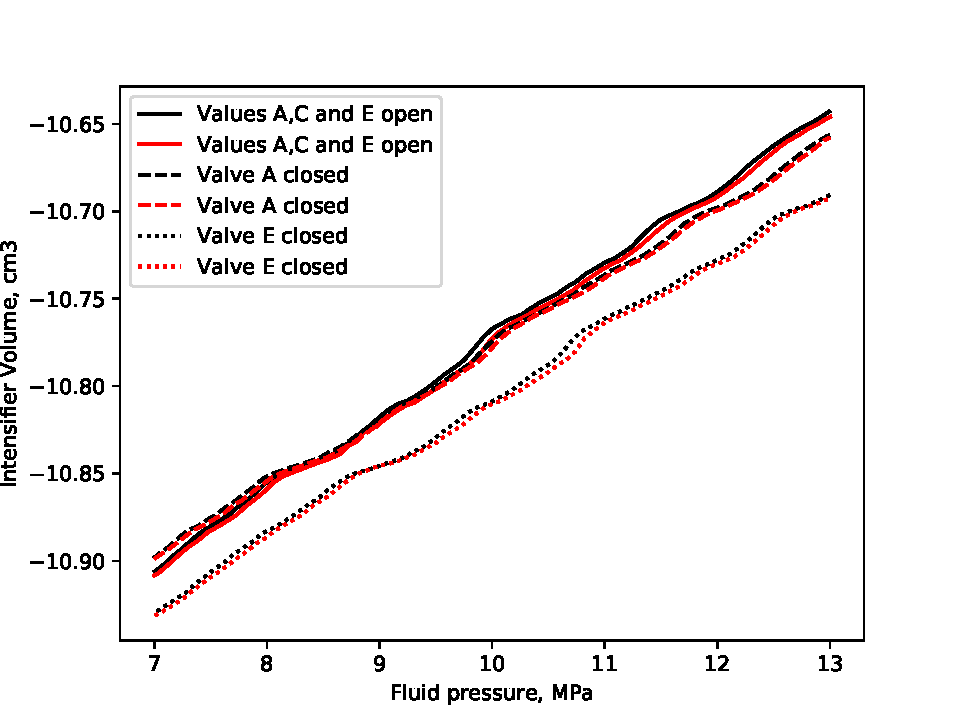
\includegraphics{figs/pfvol.pdf}
    \caption{PLACEHOLDER. The fluid volume change measured on the pore pressure intensifier due to controlled changes in fluid volume with a combination of valves open and closed.}
    \label{fig:pfcalib}
\end{figure}


\section{Modelling pore pressure diffusion}
\begin{itemize}
    \item Similar to section in my upgrade?
    \item Potentially some more detail of the equations in appendix
    \item At a minimum I need to describe the pore pressure diffusion equations and relevant boundary conditions for my experimental conditions.
    \item Show the solution to the relevant problems including plots of useful time series (log spaced) and parameters of importance (e.g. granite versus sandstone?)
    \item More details include the Laplace transform and solving for "poles" in the inverse Laplace transform.
\end{itemize}


The evolution of pore pressure in the sample over time can be modelled using the pore pressure diffusion equation, where 
\begin{equation}\label{eq:ppeqramp}
	\frac{\partial p}{\partial t} -\frac{k}{\beta_{\sigma} \mu}\frac{\partial^2 p}{\partial z^2} + \frac{B_i}{3} \frac{\partial \sigma_i}{\partial t},
\end{equation}
with initial condition
\begin{equation}
    p(z,t=0)=0,
\end{equation}
and boundary conditions
\begin{subequations}
\begin{equation}
    \left(\frac{\partial p }{\partial z}\right)_{z=0},
\end{equation}
\begin{equation}
    \beta_{\mathrm{res}}\left(\frac{\partial p }{\partial t}\right)_{z=L/2} +
    \frac{kA}{\mu}\left(\frac{\partial p }{\partial z}\right)_{z=L/2} = 0.
\end{equation}
\end{subequations}
We take an initially constant change in stress with time ($r$) followed by no change in stress after time $t_{\mathrm{end}}$,
%We assume that the change in stress with time is constant ($r$) until time $t_{\mathrm{end}}$, and then zero after:
\begin{equation}\label{eq:rampsource}
\frac{\partial \sigma_i}{\partial t} =
	\begin{cases}
		r, & 0< t \leq t_{\mathrm{end}},\\
		0, & t > t_{\mathrm{end}}.
	\end{cases}	
\end{equation}
We first normalise the system of equations using
\begin{subequations}
\begin{equation}
    t^* = t/ \tau,
\end{equation}
\begin{equation}
    z^* = z/L,
\end{equation}
\end{subequations}
where
\begin{equation}
    \tau = \frac{S_{\sigma}\mu L^2}{k}.
\end{equation}
Giving
\begin{subequations}
\begin{equation}
	\frac{\partial p}{\partial t^*} -\frac{\partial^2 p}{\partial {z^*}^2} =
	\begin{cases}
		\tau r, & 0< t^* \leq t_{\mathrm{end}}\tau =t_0,\\
		0, & t^* > t_{\mathrm{end}}\tau =t_0
	\end{cases},
\end{equation}
\begin{equation}
    p(z^*,t^*=0)=0,
\end{equation}
\begin{equation}
    \left(\frac{\partial p }{\partial z^*}\right)_{z^*=0},
\end{equation}
\begin{equation}
    \left(\frac{\partial p}{\partial t^*}\right)_{z^*=1/2} +
    h\left(\frac{\partial p}{\partial z^*}\right)_{z^*=1/2} = 0,
\end{equation}
\end{subequations}
where
\begin{equation}
    h = \frac{ALS_{\sigma}}{\beta_{\mathrm{res}}}.
\end{equation}
To solve this we apply the Laplace transform which is defined as (dropping the $^*$)
\begin{equation}
    \bar{p}(z,s) = \int_0^{\infty}e^{-st}p(z,t)dt,
\end{equation}
to get a new system of equations 
\begin{subequations}\label{eq:laplaceeqs}
\begin{equation}
	s\bar{p}(z,s) - \frac{\partial^2\bar{p}}{\partial z^2} =
	\begin{cases}
		\tau r \frac{1}{s}, & 0< t \leq t_0,\\
		\tau r \frac{1}{s} \left(1 - e^{-st_0}\right), & t > t_0
	\end{cases},
\end{equation}
\begin{equation}\label{eq:bc1}
    \left(\frac{\partial \bar{p} }{\partial z}\right)_{z=0} = 0,
\end{equation}
\begin{equation}\label{eq:bc2}
    s\bar{p}(z=1/2,s) +
    h\left(\frac{\partial p}{\partial z}\right)_{z=1/2} = 0.
\end{equation}
\end{subequations}
We solve equations \ref{eq:laplaceeqs} for $0< t \leq t_0$ and $t > t_0$ separately. First finding a particular solution for $t > t_0$
\begin{equation}
    \frac{\tau r}{s^2} \left( 1 - e^{-st_0} \right),
\end{equation}
and a solution to the homogeneous equation
\begin{equation}
    Ce^{-\sqrt{s}z} +De^{\sqrt{s}z},
\end{equation}
giving a general solution
\begin{equation}
   \bar{p} =  Ce^{-\sqrt{s}z} +De^{\sqrt{s}z} + \frac{\tau r}{s^2} \left( 1 - e^{-st_0} \right),
\end{equation}
where $C$ and $D$ are constants (in $z$) to be found. Using the boundary conditions from equation \ref{eq:bc1} and \ref{eq:bc2} and with some simplification gives
\begin{equation}\label{eq:Laplacesol}
    \bar{p} = \frac{\tau r \left( e^{-st_0} -1 \right)\left(\sqrt{s}\cosh{(\sqrt{s}z)} - \sqrt{s}\cosh{(\sqrt{s}/2)} -h\sinh{(\sqrt{s}/2)} \right)}{s^2\left(\sqrt{s}\cosh{(\sqrt{s}z)} - h\sinh{(\sqrt{s}/2)} \right)}.
\end{equation}
To find the solution the process of \cite{Hsieh1981}. The inverse Laplace transform is obtained using
\begin{equation}
    p(z,t) = \frac{1}{2\pi i}\int^{c+i\infty}_{c-i\infty}e^{st}\bar{p}(z,s)ds,\quad c \in \mathbb{R},
\end{equation}
where $s$ is complex and all the singularities lie within the contour left of the line $(c+i\infty,c-i\infty)$, with $c$ made large enough. The solution is given by the sum at the residues by Cauchy's residue theorem
\begin{equation}
    p(z,t) = \Sigma_m \mathrm{Res}(s_m),
\end{equation}
where $s_m$ are the poles of $e^{st}\bar{p}(z,s)$, and Res$(s_m)$ are the residues. There is a pole at $s=0$, and the residue is found by finding the Laurent series of the integrand and taking the coefficient of the order $z^{-1}$ term giving
\begin{equation}
    \mathrm{Res}(p,s=0) = \frac{\tau r t_0 h}{2+h}.
\end{equation}



%We get a solution to equation (\ref{eq:ppeqramp}) by applying a convolution of the solution given in equation (\ref{eq:ppsol}) with the ramp source term in equation (\ref{eq:rampsource}). Using the dimensional equation
%\begin{equation}
%\begin{split}
%	p(z,t) = \sum_{m=1}^{\infty}  \dfrac{2 \cos (2 \phi_{m} z/L) \sin (\phi_{m})}{\phi_{m} \cos (\phi_{m}) \sin (\phi_{m})}
%	\int_0^t e^{\frac{-4 \phi_{m}^{2}k}{\beta \mu L^2} (t-\lambda)}\frac{B_i}{3} \frac{\partial \sigma_i}{\partial \lambda}d\lambda\\
%- \dfrac{2}{h+2}\int_0^t  \frac{B_i}{3} \frac{\partial \sigma_i}{\partial \lambda}d\lambda
%+ \int_0^t H(t-\lambda) \frac{B_i}{3} \frac{\partial \sigma_i}{\partial \lambda}d\lambda.
%\end{split}
%\end{equation}
The solution has two parts, therefore pore pressure is expressed as
\begin{subequations}\label{eq:ppsolramp}
\begin{equation}\label{eq:ppsolrampa}
\begin{split}
	p(z,t) = \sum_{m=1}^{\infty}
	\dfrac{\cos (2 \phi_m z/L)e^{\frac{-4 \phi_{m}^{2}k}{\beta_{\sigma} \mu L^2} t} }{\phi_m^2\left((2+h)\cos (\phi_m) -\phi_m \sin (\phi_m)\right)}
	 \frac{\beta_{\sigma} \mu L^2}{k}\frac{B_i}{3}r\\
+ \dfrac{\left(6+h +12h(2+h)(\beta_{\sigma} \mu L^2/k)t -12(2+h)(z/L)^2\right)}{12(h+2)^2}\frac{\beta_{\sigma} \mu L^2}{k}  \frac{B_i}{3} r,
\end{split}
\end{equation}
for $0 < t \leq t_{\mathrm{end}}$ and
\begin{equation}\label{eq:ppsolrampb}
\begin{split}
	p(z,t) = \sum_{m=1}^{\infty} 
	\frac{\cos (2 \phi_m z/L)\left(e^{\frac{-4 \phi_{m}^{2}k}{\beta_{\sigma} \mu L^2} t} -
	e^{\frac{-4 \phi_{m}^{2}k}{\beta_{\sigma} \mu L^2} (t-t_0)} \right)}{\phi_m^2\left((2+h)\cos (\phi_m) -\phi_m \sin (\phi_m)\right)}
	\frac{\beta_{\sigma} \mu L^2}{k}\frac{B_i}{3}r \\
+ \frac{h}{h+2}\frac{\beta_{\sigma} \mu L^2}{k}  \frac{B_i}{3} r,
\end{split}
\end{equation}
\end{subequations}
for $t>t_{\mathrm{end}}$, where $z$ is normalised by the sample length $L$, $\phi_m$ are solutions of
\begin{equation}
2\phi +h\tan(\phi) =0,
\end{equation}
with
\begin{equation}
h = \frac{A\beta_{\sigma}L}{\beta_{\mathrm{res}}},
\end{equation}
$A$ is the cross-sectional area of the sample, and $\beta_{\mathrm{res}}$ is the storage of the reservoir at either end of the sample.

\section{Fitting pore pressure diffusion}
\begin{itemize}
    \item Details of procedure
    \item Inverse model for 3 parameters: $B_x$ (or $B_z$), $k$, and $\beta_{\sigma}$.
    \item Grid search to find least absolute difference between measurements and forward model.
\end{itemize}

\section{Development of method}
\begin{itemize}
    \item First experiment was not perfect and was build upon for experiment with data shown here.
    \item For example, piston friction was not properly considered and therefore small steps in applied axial load did not result in much change in load (and therefore stress) in the sample.
\end{itemize}

\section{Inversion of p and sh waves}
\subsection{group and phase velocity are not the same}
cite thomsen paper


\section{Description of experiment}
\subsection{Heat treatment}
The material used for this experiment was Westerly granite. A cylindrical sample, 40 mm in diameter and 100 mm in length was cored, with the ends ground flat and parallel to ensure parallelism within a precision of 0.02 mm. To generate open microcracks in the material, the sample was heat treated at room pressure to 600 $^{\circ}$C (past the $\alpha / \beta$ phase transition of quartz). The heating rate was 3 degrees C per minute, to minimise thermal gradients \citep{Wang2013}. The sample was left at 600 $^{\circ}$C for 3 hours, after which the temperature was decreased by 8 $^{\circ}$C per minute and then sample was left overnight to cool to room temperature. After thermal treatment, the sample expanded from an initial length of 100.00 mm to 100.90 mm and from a diameter of 40.08 mm to 40.40 mm.
\subsection{Bench top wave velocity measurements}

Wave velocity measurements were made at room  pressure in an intact sample of Westerly granite and in the same sample following thermal treatment to a maximum of 600 $^\circ$C. In the intact sample p-wave velocity was 4.9 km/s vertically and 5.2 km/s horizontally, and s-wave velocity was 2.8 km/s vertically and 2.7 km/s horizontally. After heating, p-wave velocity was 1.1 km/s vertically and 1.4 km/s horizontally, and s-wave velocity was 0.7 km/s vertically and 0.8 km/s horizontally.
